% Created 2024-08-03 Sat 16:24
% Intended LaTeX compiler: pdflatex
\documentclass[10pt]{article}
% =================================BASE====================================%
\usepackage[left=2cm,right=2cm,top=2cm,bottom=2cm]{geometry} % Marges
\usepackage[T1]{fontenc} % Nécessaire avec FrenchBabel
\usepackage[utf8]{inputenc} % Important pour symboles Francophones, é,à,etc
\usepackage{csquotes} % Recommandé par PDFLatex lors de la compilation. 

% Calligraphie
%\usepackage{pxfonts} % Met le texte ET les maths en Palatino + donne accès à des symboles math
%\usepackage{palatino} % Cette commande met seulement le texte en police palatino
\usepackage{lmodern} % Pour les maths? Lmodern pour les maths
\usepackage{cfr-lm}
% Use lmodern for sans-serif
\usepackage{mathrsfs} % Permet la command \mathscr (Lettres attachées genre) \mathscr(B)

% Bibliographie
%\usepackage[backend=bibtex,style=phys,sorting=ynt]{biblatex}
\usepackage[backend=biber,sorting=ynt,style=authoryear]{biblatex} % N'est pas utilisé par le compilateur org-mode, mais NÉCESSAIRE. Voir le fichier init.el pour changer le style. 
\addbibresource{master-bibliography.bib}


\usepackage{amsmath, amssymb, amsthm} % Symb. math. (Mathmode+Textmode) + Beaux théorèmes.
\usepackage{mathtools,cancel,xfrac} % Utilisation de boîtes \boxed{} + \cancelto{}{}, xfrac
\usepackage{graphicx, wrapfig} % Géstion des figures.
\usepackage{hyperref} % Permettre l'utilisation d'hyperliens.
\usepackage{color} % Permettre l'utilisation des couleurs.
\usepackage{colortbl} % Color tables
\usepackage[dvipsnames]{xcolor} % Couleurs avancées.

% Physique
\usepackage{physics} % Meilleur package pour physicien. 

% Style
\usepackage{lipsum} % For fun
\usepackage{tikz} % Realisation de figures TIKZ.
\usetikzlibrary{arrows.meta,bending} % Arrow heads 
\usepackage{empheq} % Boite autour de MULTIPLE équations
\usepackage{bbding}

% Français
\usepackage[french]{babel} % Environnements en Français.

\usepackage{titling} % Donne accès à \theauthor, \thetitle, \thedate

% ==============================BASE-(END)=================================%





% ================================SETTINGS=================================%
% Pas d'indentation en début de paragraphe :
\setlength\parindent{0pt}
\setlength{\parskip}{0.15cm}

% Tableaux/tabular
% Espace vertical dans les tabular/tableaux
\renewcommand{\arraystretch}{1.2}
% Couleur des tableaux/tabular
% \rowcolors{3}{violet!5}{}

% Couleurs de hyperliens :
\definecolor{mypink}{RGB}{147, 0, 255}
\hypersetup{colorlinks, 
             filecolor=mypink,
             urlcolor=mypink, 
             citecolor=mypink, 
             linkcolor=mypink, 
             anchorcolor=mypink}


% Numéros d'équations suivent les sections :
\numberwithin{equation}{section} 

% Les « captions » sont en italique et largeur limitée
\usepackage[textfont = it]{caption} 
\captionsetup[wrapfigure]{margin=0.5cm}

% Retirer l'écriture en gras dans la table des matières
\usepackage{tocloft}
\renewcommand{\cftsecfont}{\normalfont}
\renewcommand{\cftsecpagefont}{\normalfont}

% Change bullet style
\usepackage{pifont}
\usepackage{enumitem}
%\setlist[itemize,1]{label=\ding{224}}
\setlist[itemize,1]{label=\ding{239}}
\renewcommand{\boxtimes}{\blacksquare}
% ================================SETTINGS=================================%



% ==============================NEWCOMMANDS================================%
% CQFD symbol
\renewcommand{\qedsymbol}{$\hfill\blacksquare$}

% Vecteurs de base :
\newcommand{\nvf}{\vb{\hat{n}}}
\newcommand{\evf}{\vb{\hat{e}}}
\newcommand{\ivf}{\vb{\hat{i}}}
\newcommand{\jvf}{\vb{\hat{j}}}
\newcommand{\kvf}{\vb{\hat{k}}}
\newcommand{\uu}{\vb{u}}
\newcommand{\vv}{\vb{v}}
\newcommand{\ust}{\vb{u}_{\ast}}

% Physics empty spaces 
\newcommand{\short}{\vphantom{pA}}
\newcommand{\tall}{\vphantom{pA^{x^x}_p}}
\newcommand{\grande}{\vphantom{\frac{1}{xx}}}
\newcommand{\venti}{\vphantom{\sum_x^x}}
\newcommand{\pt}{\hspace{1pt}} % One horizontal pt space

% Moyenne numérique entre deux points de grilles. 
\newcommand{\xmean}[1]{\overline{#1}^x}
\newcommand{\ymean}[1]{\overline{#1}^y}
\newcommand{\zmean}[1]{\overline{#1}^z}
\newcommand{\xymean}[1]{\overline{#1}^{xy}}

% Tilde over psi
\newcommand{\tpsi}{\tilde{\psi}}
\newcommand{\tphi}{\tilde{\phi}}

% Nota Bene env : (\ding{89})
%\newcommand{\nb}{$\boxed{\text{\footnotesize\EightStarConvex}\pt \mathfrak{N. B.}}$\hspace{4pt}}
\newcommand{\nb}{\underline{{\footnotesize\EightStarConvex}\pt $\mathfrak{N.B.}$\vphantom{p}}\hspace{3pt}}

\newcommand{\exemple}{
\parbox[center]{2.2cm}{\begin{tcolorbox}[sharp corners, rounded corners=northeast, rounded corners=southeast,
colback=Violet!2, colframe=black,
size=small, width=2cm, left=-0.25pt, bottom=-0.5pt,
arc is angular, arc=2.5mm, boxrule=0.35pt, leftrule=4pt, %bottomrule=1pt,
after={\enskip}] Exemple \end{tcolorbox}}}

\newcommand{\rad}{\text{Rad}}


\newcommand{\cqfd}{\hfill$\blacktriangleleft$}

% Define the nota bene environment
\usepackage{tcolorbox}
\newtcolorbox{notabene}{
     colback=blue!5,
     colframe=black,
     boxrule=0.5pt,
     arc=2pt,
     left=5pt,
     right=5pt,
     top=5pt,
     bottom=5pt,
}


\newcommand{\cmark}{\ding{52}}
\newcommand{\xmark}{\ding{55}}
% ==============================NEWCOMMANDS================================%



% ==============================PAGE-TITRE=================================%
% Titlepage 
\newcommand{\mytitlepage}{
\begin{titlepage}
\begin{center}
{\Huge \thesubtitle \par}
\vspace{2cm}
{\Huge \MakeUppercase{\thetitle} \par}
\vspace{2cm}
RÉALISÉ DANS LE CADRE\\ D'UN PROJET POUR \par
\vspace{2cm}
{\Huge ISMER--UQAR \par}
\vspace{2cm}
{\thedate}
\end{center}
\vfill
Rédaction \\
{\theauthor}\\
\url{charles-edouard.lizotte@uqar.ca}\\
ISMER-UQAR\\
Police d'écriture : \textbf{CMU Serif Roman}
\end{titlepage}
}
% ==============================PAGE-TITRE=================================%



% =================================ENTÊTE==================================%
\usepackage{fancyhdr}
\pagestyle{fancy}
\setlength{\headheight}{13pt}
\renewcommand{\headrulewidth}{0.025pt} % Ligne horizontale en haut

\fancyhead[R]{\textit{\thetitle}}
\fancyhead[L]{\ \thepage}
\fancyfoot[R]{\textit{\theauthor}}
\fancyfoot[L]{}
\fancyfoot[C]{} 
% =================================ENTÊTE==================================%
\author{Charles-Édouard Lizotte}
\date{13/10/2023}
\title{Carnet de bord, Université McGill}
\newcommand{\thesubtitle}{Contrat Été 2023}
\hypersetup{
 pdfauthor={Charles-Édouard Lizotte},
 pdftitle={Carnet de bord, Université McGill},
 pdfkeywords={},
 pdfsubject={},
 pdfcreator={Emacs 29.4 (Org mode 9.7.8)}, 
 pdflang={French}}
\begin{document}

\mytitlepage
\tableofcontents\newpage
\section{Épaisseur nulle pour le modèle non-couplée -- \textit{<2023-10-12 Thu>}}
\label{sec:orgb54329a}

\begin{wrapfigure}[18]{l}{0.45\textwidth}\vspace{-\baselineskip} \centering
\centering
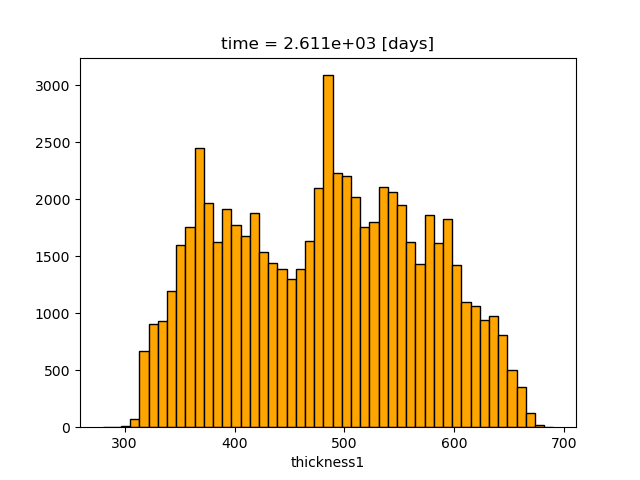
\includegraphics[width=0.45\textwidth]{figures/debuggage/2023_10_08_thickness1_histo.png}
\caption{\label{fig:org63e7290}Histograme de l'épaisseur de la première couche du dernier output avant que l'épaisseur atteingne zéro.}
\end{wrapfigure}


Comme ajouté dans le dernier rapport, le modèle \emph{shallow water} dit maintenant à quel point spatial l'épaisseur a atteint une valeur nulle.
Pour diagnostiquer l'erreur, on a maintenant un moyen d'observer ce qui se passe, comme illustré à la figure \ref{fig:org204dee2}.
Dans ce cas précis, le modèles \emph{shallow water} non couplé semble encore montrer des signes d'instabilités assez aléatoires.
En somme, nous étions parti d'une \emph{run} précédente qui avait (elle aussi) atteint une épaisseur nulle pour voir ce qui se passait.
Par contre, la \emph{run} n'a pas explosée immédiatement, ce qui vient confirmer que c'est probablement de l'erreur numérique.
À la figure \ref{fig:org204dee2}, c'est pas mal ce qu'on peut voir.
Un point bleu apparait très rapidement en haut à droite des quatres quadrants (1 \emph{output} aux deux heures). \bigskip

Malheureusement, l'histograme n'est pas très évocateur, comme il manque définitivement des pas de temps (voir fig. \ref{fig:org63e7290}).
Malgré tout, aux vue de l'animation de la figure \ref{fig:org204dee2}, je pense que c'est une erreur de type numérique.\bigskip

Principalement pour ces trois raisons : 
\begin{enumerate}
\item Ça apparaît de nulle part;
\item On voit presque un motif qui ressemble à de l'instabilité numérique dans la figure;
\item Ça se produit dans une zone où les courants sont extrêmement forts.
\end{enumerate}


\begin{figure}[!htpb]
\centering
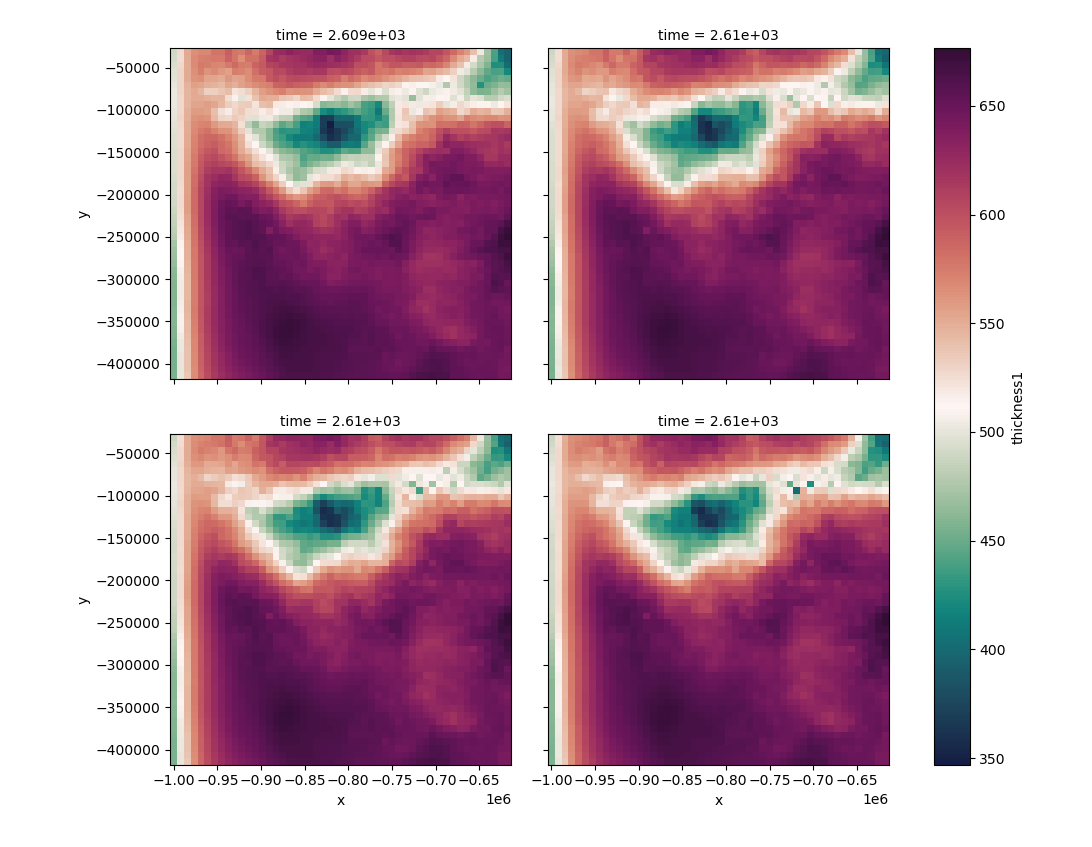
\includegraphics[width=0.7\textwidth]{figures/debuggage/2023_10_08_thickness1_last4steps.png}
\caption{\label{fig:org204dee2}Diagnostique de l'épaisseur d'une run précise du modèle \emph{shallow water}. On peut voir sur ce zoom que l'instabilité dans l'épaisseur apparait dans le haut à droite de tous les quadrant avant que le modèle s'arrête. De gauche à droite les temps -4, -3 et en bas : -2, -1.}
\end{figure}
\subsection{Solutions : Filtre de Robert plus fort? -- \textit{<2023-10-12 Thu>}}
\label{sec:org099173d}
On peut diminuer les pas de temps ou augmenter la puissance du filtre de Robert?
Il faudrait voir avec David pour ça.
pour l'instant, j'ai testé plusieurs amplitudes pour le filtre de Robert.
Les valeurs utilisées sont illustrées dans le tableau \ref{tab:orgb554ef6} et l'on y retrouve aussi le nombre de pas de temps que le modèle s'est rendu avant de lâcher à cause d'une instabilité numérique causant une épaisseur nulle. 

\begin{table}[htbp]
\caption{\label{tab:orgb554ef6}Résumé des valeurs utilisées comme filtre de Robert, dans le but de « smoother » les instabilités numériques.}
\centering
\begin{tabular}{ccccc}
\hline
Robert & \(\sfrac{L_d}{dx}\) & max(c\textsubscript{bc}) & \(\abs{\vb{\tau}}\) & Temps\\
{[} -- ] & {[} -- ] & {[} \(\sfrac{m}{s}\) ] & {[} \(\sfrac{N}{m^2}\) ] & {[} -- ]\\
\hline
\hline
0.001 & 5.363 & 2.6 & 0.1 & 362 712 et 362 664\\
0.005 & 5.363 & 2.6 & 0.1 & 613 656\\
0.010 & 5.363 & 2.6 & 0.1 & 445 904\\
0.050 & 5.363 & 2.6 & 0.1 & 633 240\\
0.100 & 5.363 & 2.6 & 0.1 & 746 663\\
\hline
\hline
\end{tabular}
\end{table}

Donc, je pourrais dire que ça n'a pas vraiment marché.
On va passer à une autre solution.
\subsection{Solution : pas de temps plus faible? -- \textit{<2023-10-13 Fri>}}
\label{sec:org8df59a4}

Une autres solution proposée par David.
Si notre diagnostique d'erreur numérique est bon, ça devrait régler le problème.
J'ai donc relancé les tests à plusieurs couches pour voir si l'on arrivait à quelque chose de concluant.
Tous ces tests sont réalisés avec un pas de temps de 200 secondes au lieu du 300 secondes généralement utilisé.\bigskip

Après avoir tenté l'expérience, j'ai vu que le pas de temps ne change arbitrairement rien.
Au fond, il semble qu'il y ait des incursions lorsque deux « blobs » se séparent et il faudrait trouve un moyen de gérer ces incursions.
Un résumé des expériences se retrouve dans le tableau \ref{tab:org3a1bbb1}.

\begin{table}[htbp]
\caption{\label{tab:org3a1bbb1}Résumé des expériences lancées avec un pas de temps de 200 secondes au lieu de 300.}
\centering
\begin{tabular}{cccc}
\hline
Nombre de couches & min(\(\sfrac{L_d}{dx}\)) & max(c\textsubscript{bc}) & Dernier pas de temps\\
\hline
\hline
3 & 5.363 & 2.6 & 583 092\\
4 & 3.488 & 2.5 & 391 284\\
5 & 2.459 & 2.5 & 226 584\\
6 & 1.852 & 2.5 & 133 056\\
\hline
\end{tabular}
\end{table}

Mentionnons que les incursions se produisent généralement sur le bord ouest ou à la jonction entre deux tourbillons.
Par exemple, à la figure \ref{fig:thickness-close} on observe une incursion à l'intérieur du domain pour l'expérience à trois couches.
Tandis qu'on observe une incusrion à la frontière pour l'expérience à 4 couches (Voir figure \ref{fig:thickness-close2}).


\begin{figure}[!htpb]
\centering
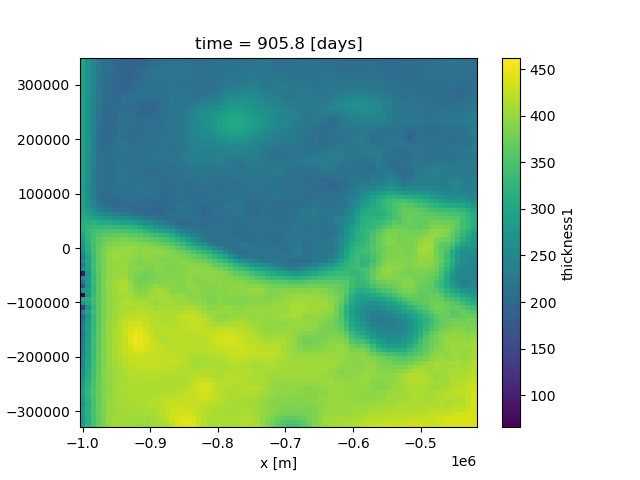
\includegraphics[width=0.45\textwidth]{figures/debuggage/2023_10_16_thickness_closeup.png} 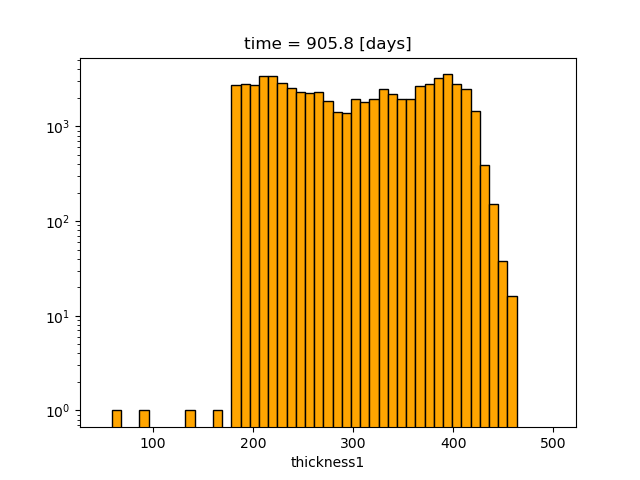
\includegraphics[width=0.45\textwidth]{figures/debuggage/2023_10_16_thickness_histo2.png}
\caption{« Snapshot » de l'épaisseur de la couche supérieure en zoom sur la zone où cette dernière devient nulle. Et histograme de l'épaisseur de la première couche au même moment. Tirée de l'expérience à 4 couches.}
\label{fig:thickness-close}
\end{figure}

\begin{figure}[!htpb]
\centering
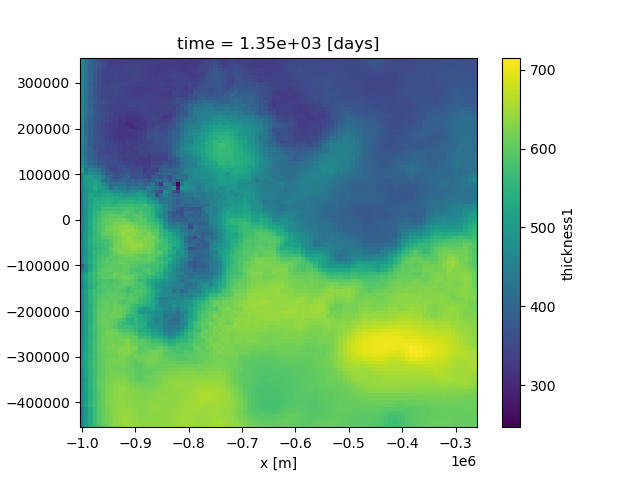
\includegraphics[width=0.45\textwidth]{figures/debuggage/2023_10_16_thickness_closeup2.png}
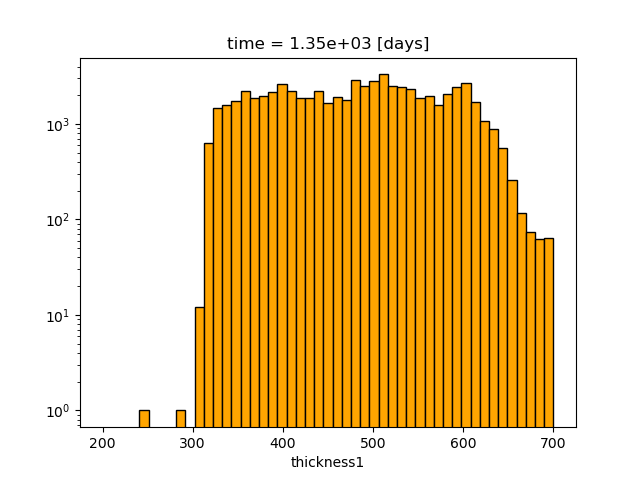
\includegraphics[width=0.45\textwidth]{figures/debuggage/2023_10_16_thickness_histo.png}
\caption{ « Snapshot » de l'épaisseur de la couche supérieure en zoom sur la zone où cette dernière devient nulle. Et histograme de l'épaisseur de la première couche au même moment. Tirée de l'expérience à 3 couches.}
\label{fig:thickness-close2}
\end{figure}
\subsection{Le besoin d'un transfert de masse et/ou d'un Laplacien sur l'épaisseur des couches?}
\label{sec:org6d6eaa6}
\section{Retour rapide sur la « partial slip » -- \textit{<2023-10-13 Fri>}}
\label{sec:orgccf7cf6}
La \emph{partial} et la \emph{free slip} est maintenant controlée par la même sous-routine \emph{partial free slip.f90}.
Tout passe maintenant par le paramètre « \(\alpha\) » qui décrit la proportion de la dérivée qui doit passer dans l'équation
\begin{equation}
   \eval{\pdv{u}{y} - \alpha \cdot u = 0\hspace{0.2cm}}_{\pt\forall\pt y\pt \in\pt \qty{0,\pt L_y}}.
\end{equation}
Donc, si l'on fixe une valeur nulle à « \(\alpha\) », on obtient une condition \emph{free slip}.
Simple comme ça. 
\section{« Spin up » de la dérive de Stokes -- \textit{<2023-10-12 Thu>}}
\label{sec:org50089a6}

\begin{wrapfigure}[14]{r}{0.65\textwidth}
\vspace{-\baselineskip}
\begin{center}
\begin{tikzpicture}[scale=1.4]
   % Rectangles :
   \fill [BurntOrange!10] (0,0) rectangle (2,3) ;
   \fill [BurntOrange!18] (2,0) rectangle (4,3) ;
   \fill [BurntOrange!26] (4,0) rectangle (6,3) ;
   %
   \draw (1,2.75) node [] {Spin up};
   \draw (3,2.75) node [] {Ramp};
   \draw (5,2.75) node [] {Couplé};
   %
   \draw [->] (0,0) -- (6.25,0);
   \draw [->] (0,0) -- (0,3.25);
   \draw [dotted] (0,2.5) -- (6,2.5);
   \draw [thick, BurntOrange!50!red!90] (0,0.01) -- (2,0.01) -- (4,2.5) -- (6,2.5);
   \draw (0,2.5) node [left] {1};
   \draw (0,0) node [left] {0};
   \draw (0,1.25) node [rotate=90, above] {Rampe};
   \draw (2,0) node [below] {2 jours};
   \draw (4,0) node [below] {1 mois};
   \draw (6,0) node [below] {Temps};
\end{tikzpicture}
\end{center}
\caption{\label{org2e222ae}Illustration conceptuelle de la rampe pour éviter le \emph{spin up} du modèle de vagues.}
\end{wrapfigure}

En somme, le modèle de vagues a un \emph{spin up} extrême, pas en terme d'amplitude, mais en terme de vitesse et ça fait tout sauter -- l'épaisseur de la première couche atteint 0 en moins de 90 pas de temps.
Donc, ce qu'on va faire, c'est une rampe différente que \emph{saute par dessus} le \emph{spin up} du modèle de vagues.
Quelque chose qui ressemble à la figure \ref{org2e222ae}. \bigskip

Bien que je croyais que cette solution serait suffisante, il semble que la dérive de Stokes soit encore trop forte.
Nous allons donc essayer d'autres avenues dans les sections suivantes. 
\section{Problème de dérive de Stokes}
\label{sec:org1dd1adb}
Après avoir tenté la solution proposée dans la section précédente, on voit qu'il faudra bien plus qu'une rampe pour satisfaire le modèle \emph{shallow water}.
Sommairement, le modèle \emph{shallow water} ne tient pas le coups car la dérive de Stokes induit un gradient extrême dans la partie droite du domaine (Voir figure \ref{fig:org11a1dd7}).

\begin{figure}[htbp]
\centering
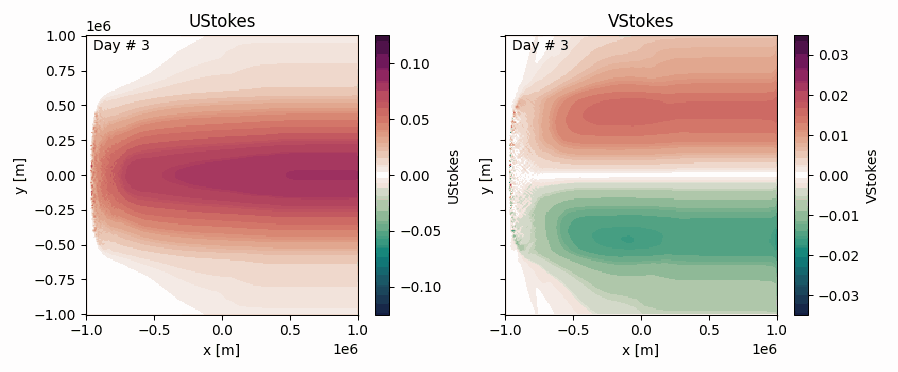
\includegraphics[width=.9\linewidth]{figures/debuggage/2023_10_13_UStokes.png}
\caption{\label{fig:org11a1dd7}Figure instantanée du profil associé au transport de Stokes après trois jours.}
\end{figure}

Lors de ma maîtrise, nous n'avions pas ce problème, car les zones primaires de productions de vagues (ZPPV) étaient à l'extérieur du domaine périodique, de sorte qu'on évitait le gradient élevé dans cette zonne (Voir figure \ref{fig:org664f63b})

\begin{figure}[!htpb]
\centering
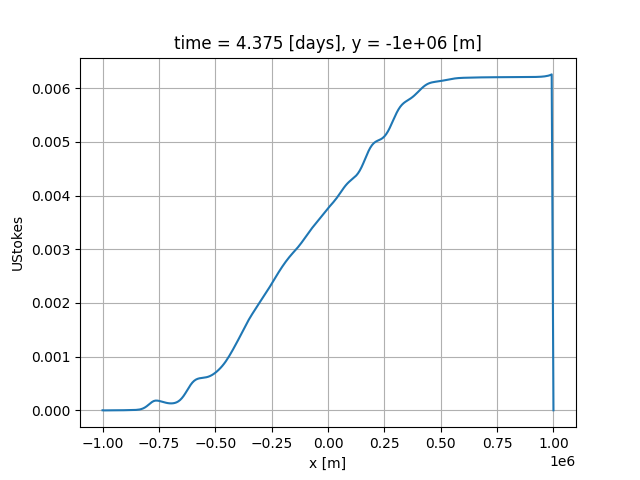
\includegraphics[width=0.5\textwidth]{figures/debuggage/2023_10_13_Stokes_coupe.png}
\caption{\label{fig:org664f63b}Coupe horizontale du transport de Stokes après 4 jours.}
\end{figure}

Le même délire arrive aussi avec le \(\tau_{wave}\) et \(\tau_{dissipation}\), mais à moindre échelle.
\section{Solutions à l'étude -- \textit{<2023-10-13 Fri>}}
\label{sec:org8de21de}

\begin{itemize}
\item \textbf{Ramener le coefficient de réflection aux murs dans le modèle de vagues.}
Ça permettrait d'avoir des vagues déjà formées dans la partie ouest et ça viendrait diminuer le chaos dans la zone primaire de production de vagues.\bigskip

\item \textbf{Essayer un schéma de vent différent}, tel que
\begin{equation}
  \tau_{atm} = \qty(\frac{\tau_0}{2})\cdot \qty(1-\cos \frac{2\pi y}{L_y})\cdot \qty(\sin \frac{\pi x}{L_x} ).
\end{equation}
De cette manière, le gradient de vent devrait changer aussi.
Ça devrait avoir été testé cette fin de semaine.
\end{itemize}



\begin{itemize}
\item \textbf{Diminuer ou moyenner une partie de la grille de Wavewatch}.
Cette solution nous permettrait aussi de rouler le modèle Wavewatch plus rapidement.
Il faudrait seulement avoir un genre de stencil qui moyenne chaque partie, mais c'est facilement faisable.
\end{itemize}


\begin{figure}[h!]
\begin{center}
\begin{tikzpicture}
% Big grid
\fill [blue!5] (0,0) rectangle (3,3);
\fill [blue!5] (3,3) rectangle (6,6);
% Grid
\draw (0,0) rectangle (6,6) ;
\draw [dotted] (0,0) grid (6,6) ;
\draw [step=3.0] (0,0) grid (6,6) ;
% Coordinates 
\foreach \x in {1,2,3}
\foreach \y in {1,2,3}
{\draw (\x-0.5,\y-0.5) node [] {1,1};}
%
\foreach \x in {4,5,6}
\foreach \y in {1,2,3}
{\draw (\x-0.5,\y-0.5) node [] {2,1};}
%
\foreach \x in {1,2,3}
\foreach \y in {4,5,6}
{\draw (\x-0.5,\y-0.5) node [] {1,2};}
%
\foreach \x in {4,5,6}
\foreach \y in {4,5,6}
{\draw (\x-0.5,\y-0.5) node [] {2,2};}
%
\draw [red] (2,2) rectangle (5,5) ;
\fill [red, opacity=0.3] (3,3) rectangle (4,4);
\end{tikzpicture}
\end{center}
\caption{\label{org0fa041e}« Stencil » utilisé pour obtenir le champs aux plus grandes échelles.}
\end{figure}



\newpage
\subsection{Résultats -- \textit{<2023-10-16 Mon>}}
\label{sec:org04deaab}

\subsubsection{Enlever la dérive de Stokes}
\label{sec:orgd57bc15}
Ce test nous a permis de voir qu'au fond ce sont les variations dans la zone primaire de production de vagues qui viennent mettre à mal la circulation.
Même si la dérive de Stokes est abscente, on a toujours le même problème avec la variation de l'interface.
On se souvient que
\begin{align}
   && \boldsymbol{\tau}_{oc} = \underbrace{\rho_{atm} |\uu_*|\uu_*\tall}_\text{F. velocity} \ - \underbrace{\qty(\boldsymbol{\tau}_{in} - \boldsymbol{\tau}_{ds})\tall}_\text{Champ de vagues} && \text{où} && \uu_* \equiv c_d(x,y)\cdot\uu_{10} &&
\end{align}
comme illustré dans \autocite{breivik_al_2015}.
Mentionnons que \(c_d(x,y)\) est dépendant du champ de vagues. 
\begin{center}
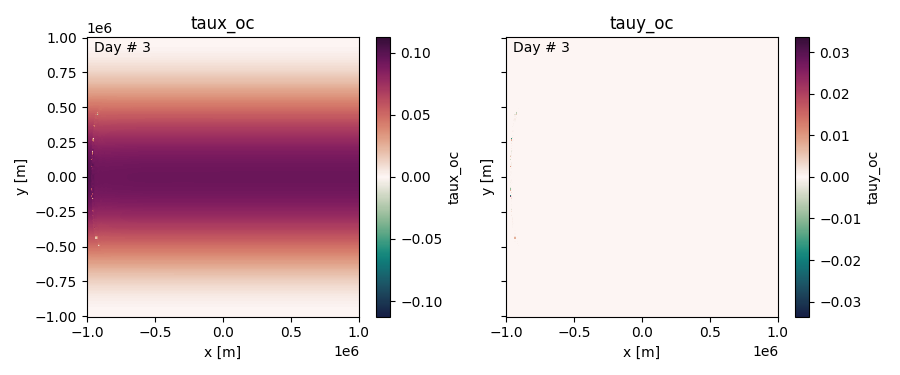
\includegraphics[width=.9\linewidth]{figures/debuggage/2023_10_16_nostokes_tauoc.png}
\end{center}
\subsubsection{Changer le type de vent}
\label{sec:org64dcd81}
J'ai implémenté le nouveau schéma pour le vent, mais sans succès

\begin{center}
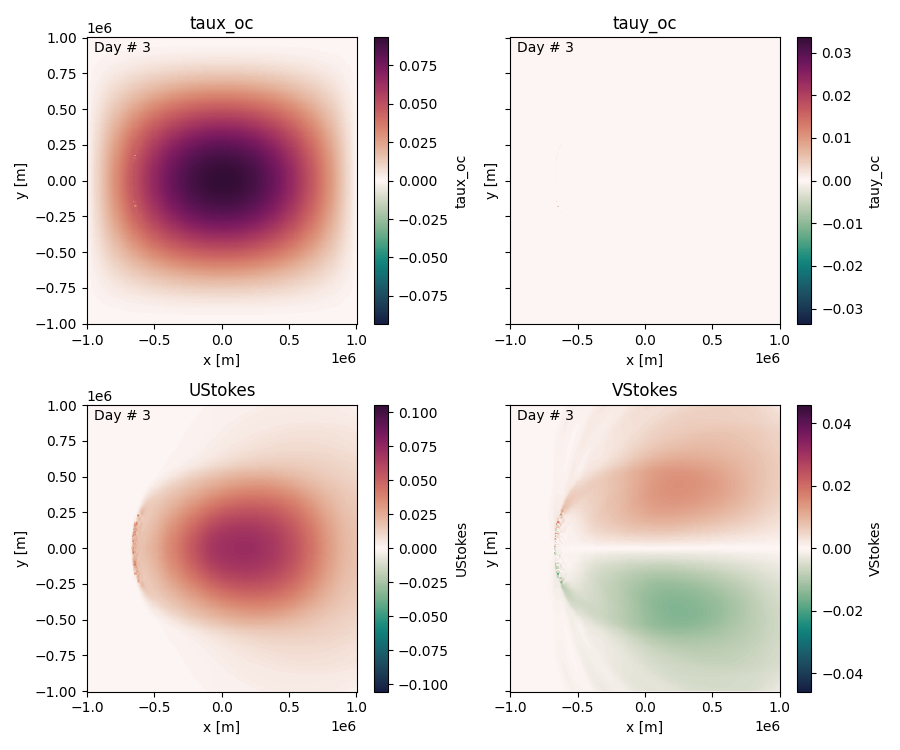
\includegraphics[width=.9\linewidth]{figures/debuggage/2023_10_16_ramp_tauETUstokes.png}
\end{center}



\printbibliography
\end{document}
